\newpage
\section{ワイヤ駆動式魚ロボットの開発}
\subsection{本研究の目的}
初めに,本研究の目的について述べる.先行研究では屈曲可能な胴体を持ち,柔軟外皮を装着して完全防水を可能にした魚ロボットの開発に成功した.しかし,リンクと外皮に隙間ができてしまい,
リンクの動きを外皮にうまく伝えることができなかった.そこで本研究では魚らしいしなやかな動きを可能にするワイヤ駆動式の魚ロボットをベースにリンクと外皮をうまく追従させ,リンクの動き
を外皮にうまく伝えることができるロボットの開発を目指す.そして外皮による遊泳性能の向上を図る.

\subsection{動作原理}
ここでは本研究で開発した魚ロボットの動作原理を記す.動作原理としてはサーボモータにプーリを取り付け,プーリを回転させることで胴体部に配したワイヤを巻き取る.ワイヤは骨格リンクに
設けられた穴を通って尾びれ付け根まで伸びており,ワイヤを巻き取ることによって胴体部を屈曲させることができる.それを左右に繰り返すことで遊泳を可能にする.

 \begin{figure}[htbp]
    \centering
    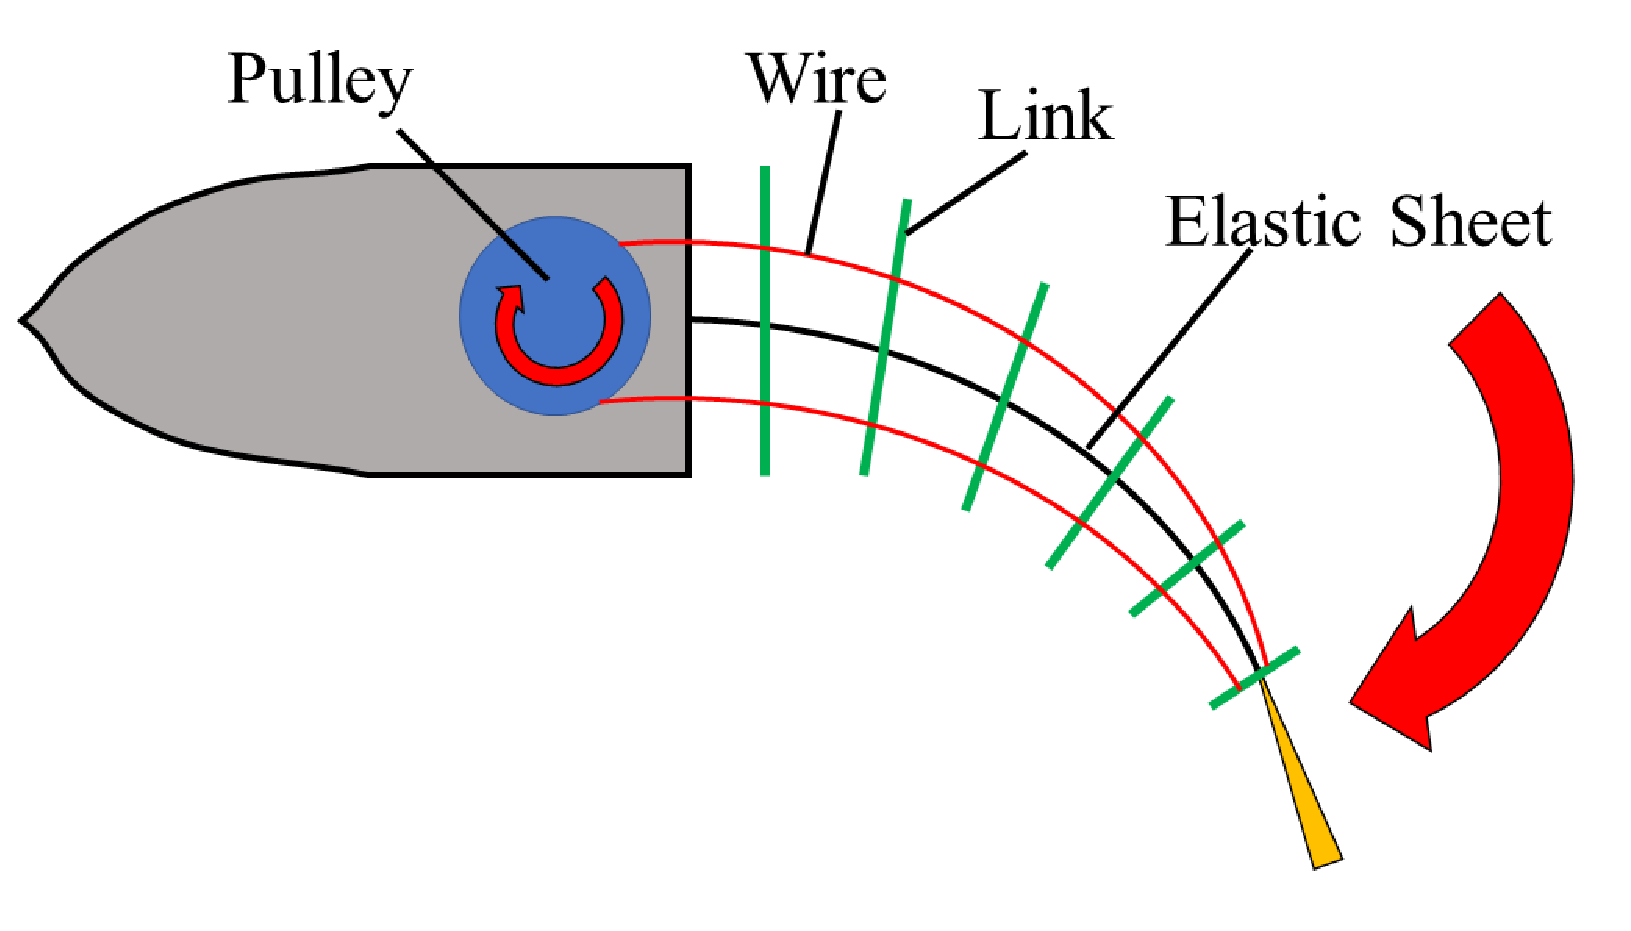
\includegraphics[width=0.8\linewidth]{/Users/watanabe_shouta/2024_graduation_thesis/picture/waiyakudou.eps}
    \caption{ワイヤ駆動のイメージ}
    \label{fig:waiyakudou}
 \end{figure}

 \subsection{試作機の作成}
 本機体の作製にあたり,まずは昨年度の先行研究を参考にして試作機を作製した.図に外観を,図に構造を示す.